% --------------------------------------------------------------------------
% Formatvorlage für Diplomarbeiten der FHWT
% --------------------------------------------------------------------------
% 	Angelehnt an die Word-Vorlage von Herrn Stührenberg
% 	Download unter http://www.atlando.de/fhwt.htm
%
% 	erstellt von Stefan Macke. 22.10.2007
% 	http://blog.stefan-macke.de
%   
%   Genutzt und angepasst auf utf8 von Johannes Dielmann 

% Meta-Informationen -------------------------------------------------------
%	Informationen über das Dokument, wie z.B. Titel, Autor, Matrikelnr. etc
%	werden in der Datei _Meta.tex definiert und können danach global
%	verwendet werden.
% --------------------------------------------------------------------------
% Informationen ------------------------------------------------------------
% 	Definition von globalen Parametern, die im gesamten Dokument verwendet
% 	werden k�nnen (z.B auf dem Deckblatt etc.).
% --------------------------------------------------------------------------
\newcommand{\titel}{Uebersetzen von Schrittmotorprotokollen}
\newcommand{\untertitel}{Entwurf eines Hardware�bersetzers}
\newcommand{\art}{Praxisbericht}
\newcommand{\fachgebiet}{Mess- und Sensortechnik}
\newcommand{\autor}{Johannes Dielmann}
\newcommand{\studienbereich}{Technik}
\newcommand{\matrikelnr}{515956}
\newcommand{\erstgutachter}{Prof. Dr. Carstens-Behrens}
\newcommand{\zweitgutachter}{Prof. Dr. }
\newcommand{\jahr}{2012}

% Eigene Befehle und typographische Auszeichnungen f�r diese
\newcommand{\todo}[1]{\textbf{\textsc{\textcolor{red}{(TODO: #1)}}}}

\newcommand{\AutorZ}[1]{\textsc{#1}}
\newcommand{\Autor}[1]{\AutorZ{\citeauthor{#1}}}

\newcommand{\NeuerBegriff}[1]{\textbf{#1}}

\newcommand{\Fachbegriff}[1]{\textit{#1}}
\newcommand{\Prozess}[1]{\textit{#1}}
\newcommand{\Webservice}[1]{\textit{#1}}

\newcommand{\Eingabe}[1]{\texttt{#1}}
\newcommand{\Code}[1]{\texttt{#1}}
\newcommand{\Datei}[1]{\texttt{#1}}

\newcommand{\Datentyp}[1]{\textsf{#1}}
\newcommand{\XMLElement}[1]{\textsf{#1}}


% Abk�rzungen mit korrektem Leerraum
\newcommand{\vgl}{Vgl.\ }
\newcommand{\ua}{\mbox{u.\,a.\ }}
\newcommand{\zB}{\mbox{z.\,B.\ }}
\newcommand{\bs}{$\backslash$}



% Dokumentenkopf -----------------------------------------------------------
% 	Diese Vorlage basiert auf "scrreprt" aus dem koma-script.
%	Die Option draft sollte beim fertigen Dokument ausgeschaltet werden.
% --------------------------------------------------------------------------
\documentclass[
	11pt,					% Schriftgröße
	DIV10,
	german,					% für Umlaute, Silbentrennung etc.
	a4paper,         		% Papierformat
	oneside,				% einseitiges Dokument
	titlepage,				% es wird eine Titelseite verwendet
	final					% Status des Dokuments (final/draft)
]{scrreprt}

% Benötigte Packages -------------------------------------------------------
%	Weitere Packages, die benötigt werden, sind in die Datei Packages.tex
%	"ausgelagert", um die Vorlage möglichst übersichtlich zu halten.
% --------------------------------------------------------------------------
\input{Packages}

% Erstellung eines Index und Abkürzungsverzeichnisses aktivieren -----------
\makeindex
\makenomenclature


% Kopf- und Fußzeilen, Seitenränder etc. -----------------------------------
% Zeilenabstand ------------------------------------------------------------
%\onehalfspacing

% Seitenränder -------------------------------------------------------------
%\geometry{paper=a4paper,left=30mm,right=40mm,top=10mm,bottom=65mm}
%\geometry{paper=a4paper,left=35mm,right=35mm,top=30mm,bottom=40mm}

%
%% Kopf- und Fußzeilen ------------------------------------------------------
%\pagestyle{scrheadings}
%
%% Kopf- und Fußzeile auch auf Kapitelanfangsseiten -------------------------
%\renewcommand*{\chapterpagestyle}{scrheadings}
%
%% Schriftform der Kopfzeile ------------------------------------------------
%\renewcommand{\headfont}{%
%\normalfont
%}
%
%% Kopfzeile ----------------------------------------------------------------
%\ihead{\large{\textsc{\titel}}\\ \small{\untertitel} \\[2ex] \textit{\headmark}}
%\chead{}
%\ohead{\includegraphics[scale=0.25]{RAC_Logo.jpg}}
%%
%\setlength{\headheight}{21mm} % Höhe der Kopfzeile
%\setheadwidth[0pt]{textwithmarginpar} % Kopfzeile über den Text hinaus verbreitern
%\setheadsepline[text]{0.4pt} % Trennlinie unter Kopfzeile
%
%% Fußzeile -----------------------------------------------------------------
%\ifoot{\autor}
%\cfoot{}
%\ofoot{\pagemark}


% erzeugt ein wenig mehr Platz hinter einem Punkt --------------------------
\frenchspacing 

% Schusterjungen und Hurenkinder vermeiden
\clubpenalty = 10000
\widowpenalty = 10000 
\displaywidowpenalty = 10000


% Quellcode-Ausgabe formatieren --------------------------------------------
\lstset{numbers=left, numberstyle=\tiny, numbersep=5pt, breaklines=true}
\lstset{emph={square}, emphstyle=\color{red}, emph={[2]root,base}, emphstyle={[2]\color{blue}}}

% Fußnoten fortlaufend durchnummerieren ------------------------------------
%\counterwithout{footnote}{chapter}



% Eigene Definitionen für Silbentrennung
\hyphenation{Laser-er-fass-ungs-system Haupt-ein-satz-ge-bie-te}


% Das eigentliche Dokument -------------------------------------------------
%	Der eigentliche Inhalt des Dokuments beginnt hier. Die einzelnen Seiten
%	und Kapitel werden in eigene Dateien ausgelagert und hier nur inkludiert.
% --------------------------------------------------------------------------
\begin{document}

% auch subsubsection nummerieren
\setcounter{secnumdepth}{3}
\setcounter{tocdepth}{3}

\ofoot{}
\thispagestyle{plain}
\begin{titlepage}

\begin{center}

\huge{\textbf{\textsc{\titel}}}\\[1.5ex]
\LARGE{\textbf{\untertitel}}\\[4ex]
\LARGE{\textbf{\art}}\\[1.5ex]
\Large{im Fachgebiet \fachgebiet}\\[6ex]

\includegraphics[scale=0.6]{RAC_Logo.jpg}\\[3ex]

\normalsize
\begin{tabular}{w{5.4cm}p{6cm}}\\
 vorgelegt von:	 & \quad \autor\\[1.2ex]
 Studienbereich: & \quad \studienbereich\\[1.2ex]
 Matrikelnummer: & \quad \matrikelnr\\[1.2ex]
 Erstgutachter:         & \quad \erstgutachter\\[1.2ex]
 %Zweitgutachter:         & \quad \zweitgutachter\\[3ex]
\end{tabular}

\copyright\ \jahr\\[1.5ex]

\end{center}

\singlespacing
\small
\noindent Dieses Werk einschließlich seiner Teile ist \textbf{urheberrechtlich geschützt}. Jede Verwertung außerhalb der engen Grenzen des Urheberrechtgesetzes ist ohne Zustimmung des Autors unzulässig und strafbar. Das gilt insbesondere für Vervielfältigungen, Übersetzungen, Mikroverfilmungen sowie die Einspeicherung und Verarbeitung in elektronischen Systemen.

\end{titlepage}

%\section*{Zusammenfassung}
\label{sec:Zusammenfassung}
\todo{besser schreiben!} Im Praxisprojekt wurde eine gegebene Aufgabe selbstständig umgesetz. Dabei wurde Hardware unter anderem in Form von Platinenlayouts entwickelt, benötigte Bauteile recherchiert und bestellt, der Aufbau verändert und verbessert. Es wurde Software entwickelt und auftrende Probleme gelöst.

\section*{Abstract}
\label{sec:Abstract}
\todo{WTH is an abstact??}

\ofoot{\pagemark}

% Seitennummerierung -------------------------------------------------------
%	Vor dem Hauptteil werden die Seiten in großen römischen Ziffern 
%	nummeriert...
% --------------------------------------------------------------------------
\pagenumbering{Roman}
%\maintoc
\tableofcontents								% Inhaltsverzeichnis

% Abkürzungsverzeichnis ----------------------------------------------------
\nomenclature{SCSI}{Small Computer System Interface}
		
\label{sec:Glossar}		
\printnomenclature

\listoffigures						% Abbildungsverzeichnis
\listoftables						% Tabellenverzeichnis
\renewcommand{\lstlistlistingname}{Codeverzeichnis}
\lstlistoflistings					% Listings-Verzeichnis

% ...danach in normalen arabischen Ziffern ---------------------------------
\clearpage
\pagenumbering{arabic}
% Inhalt -------------------------------------------------------------------
%	Hier können jetzt die einzelnen Kapitel inkludiert werden. Sie müssen
%	in den entsprechenden .TEX-Dateien vorliegen. Die Dateinamen können
% 	natürlich angepasst werden.
% --------------------------------------------------------------------------
\chapter{Einleitung}
\label{cha:Einleitung}
Ein 3D-Laserscanner bietet vielfältige Möglichkeiten und Einsatzgebiete. Die Haupt-einsatzgebiete finden sich in der Bauteileprüfung, zur Erstellung von Finite-Elemente-Daten in Verbindung mit Bauteilanalyse, zur Erstellung von 3D-Daten, zur Kontrolle von Zubehörteilen, zur Archivierung in Museen und Forschungseinrichtungen, zum Reverse-Engineering und in vielen weiteren Gebieten.\\
Im Besitz der Fachhochschule befand sich ein komplettes 3D-Lasererfassungssystem. Dazu gehörten eine Erfassungssoftware, ein 3D-Laserscanner und ein Drehtisch. Bisher mussten, um eine Aufnahme zu tätigen, alle Komponenten zueinander passen. Der Drehtisch in diesem System war jedoch ein Eigenbau der Fachhochschule und die darin verbaute Drehtischsteuerung nicht kompatibel zu denen von der Erfassungssoftware unterstützten Drehtischsteuerungen.\\
Mittels eines Mikrocontrollers sollte der vorhandene Aufbau so erweitert werden, dass der Drehtisch von der Software angesteuert werden konnte und so der volle Umfang des Systems nutzbar gemacht werden. Dabei waren folgende Vorgaben zu realisieren. Die Höhenverstellung des Drehtisches sollte genutzt werden können und die verbauten Endschalter ihre vorhergesehene Funktion erfüllen. 
Der Mikrocontroller sollte sich mit mehreren Tastern bedienen lassen und über ein LC-Display verfügen, welches den aktuellen Status anzeigt. Mit einer Schritt-für-Schritt-Anleitung sollte es auch für Studenten und Mitarbeiter der Fachhochschule möglich sein, schnell und einfach eine Aufnahme durchzuführen. Die Daten dieser Aufnahme sollten exportiert und in z.B. CAD-Software genutzt werden können. \\
Der Aufbau der Arbeit gliedert sich im Wesentlichen in die Vorstellung der Vorhanden Hard- und Software, den chronologischen Arbeitsablauf während des Projektes, ein Kapitel das Probleme und deren Lösungen aufzeigt, in ein Fazit und mögliche zukünftige Verbesserungen. Im Anhang befindet sich eine Schritt-für-Schritt-Anleitung die es Laien ermöglicht 3D-Modelle aufzunehmen und zu exportieren.
 		% Motivation und Ziel
%\chapter{Begriffe und Komponenten}
\label{cha:Begriffe}
\todo{Besseres Bild! Schema? Bessere Beschriftung!}
\begin{figure}[htb]
\centering
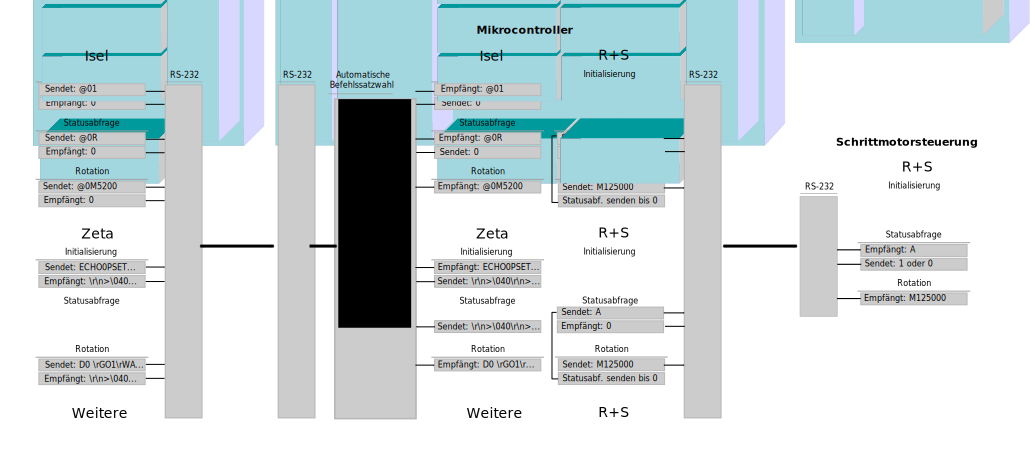
\includegraphics[width=\textwidth]{Uebersicht.jpg}
\caption{Überblick des Arbeitsplatz}
\label{fig:Übersicht}
\end{figure}
\todo{Bessere Überschrift!}
\todo{ Fußnoten für Komponenten, Hersteller und Websites}
\todo{ Komponenten auf Abbildung erwähnen!}
\section{Kopmonenten zur Erfassung}
\subsection{Lasererfassungssystem VI-900}
Das Lasererfassungsystem VI-900 der Firma Minolta besteht aus einem Lasertriangulator und einer Kamera. Das System lässt sich über eine SCSI Schnittstelle ansprechen und konfigurieren. Zur mobilen Nutzung kann das Gerät auch auf der Rückseite bedient werden. Aufgenommene Daten können auf einer CF-Karte gespeichert werden. Im Projekt wurde jedoch lediglich die Ansteuerung via SCSI genutzt.
\subsection{RapidForm2004}

\section{Drehtisch}
Der Drehtisch ist eine Eigenkonstruktion der Werkstatt des RheinAhrCampus. Er besteht aus einer massiven Edelstahl Arbeitsplatte, welche auf 4 Füßen ruht. Aus dieser ist eine \todo{Welche form??} ausgeschnitten. In diesem Ausschnitt befindet sich, auf einem Zweischienensystem gelagert, der Drehtisch. Mit dem Schienensystem lässt der Drehtisch sich in der Vertikalen positionieren. Mit einem Schrittmotor lässt sich der Drehtisch in der Höhe verstellen. Ein weiterer Schrittmotor ist für die Drehung des Tisches zuständig. \todo{Getriebe erklären!}  
\subsection{Schrittmotoren}
\todo{Motoren beschreiben!}
\subsection{Schrittmotorkarten}
Die Ansteurung für den Drehtisch besteht aus einem 19"-Rack. In diesem ist ein ATX-PC-Netzteil verbaut. Außerdem sind 2 Einschubkarten der Firma R+S vorhanden. Die Karten sind sogenannte Stepper-Karten. Diese übernehmen komfortabel die Ansteuerung der beiden Schrittmotoren. Mittels RS-232 Schnittstelle lassen sich die Karten konfigurieren und ansteuern. Die Konfiguration und Ansteuerung erfolgt über einen vorgegeben ASCII Befehlssatz. Außerdem können 2 oder mehr Karten als "Daisy-Chain" zusammengeschaltet werden. 
\todo{Daisy-Chain erklären und Konfiguration genauer beschreiben.}
\section{Mikrocontroller}
\subsection{Entwicklungsumgebung}
\subsection{Entwicklerboard STK500}
Um den eingesetzten Mikrocontroller zu programmieren und die Programmierung zu überprüfen wurde mir das Entwicklerboard STK500 der Firma ATMEL zur Verfügung gestellt. Das Board enthält mehrere Mikrocontroller Steckplätze, 2 Serielle Schnittstellen, 8 Taster, 8 LEDs, 2 Erweiterungsports, ein integriertes Programmiersystem \todo{besserer Name!} und mehrere Jumper zum konfigurieren des Boards.\\
Von den beiden seriellen Schnittstellen kann die eine zur Programmierung des Mikrocontroller verwendet werden. Die andere kann zur Kommunikation mit dem Mikrocontroller genutzt werden.\\
Auf dem Board stehen 5 10 polige Stiftleisten 
\footnote{Eine Stiftleiste (engl. pin header) ist ein Steckverbinder mit mehreren in Reihe angeordneten Stiftkontakten, der auf Leiterplatten in der Elektronik Verwendung findet. Sie hat den Zweck, eine Verbindung mit vielen Kontakten von einer Platine zu einer anderen oder zu peripheren Baugruppen herzustellen, meist mit Hilfe von Flachbandkabeln und Pfostenverbindern oder einer Buchsenleiste. \cite{wiki_pinh} }
zur Verfügung. Diese sind direkt mit dem Mikrocontroller verbunden und können über Flachbandkabel an Peripherie wie z.B. Taster, LED und LC-Displays angeschlossen werden.
\subsection{AVRISP mkII}
	% Begriffe
\chapter{Vorstellung der vorhandenen Hardware}
\label{sec:Hardware}
Die Hardware besteht im Wesentlichen aus den Komponenten in Abbildung \ref{fig:Übersicht}.
\begin{figure}[htb]
\centering
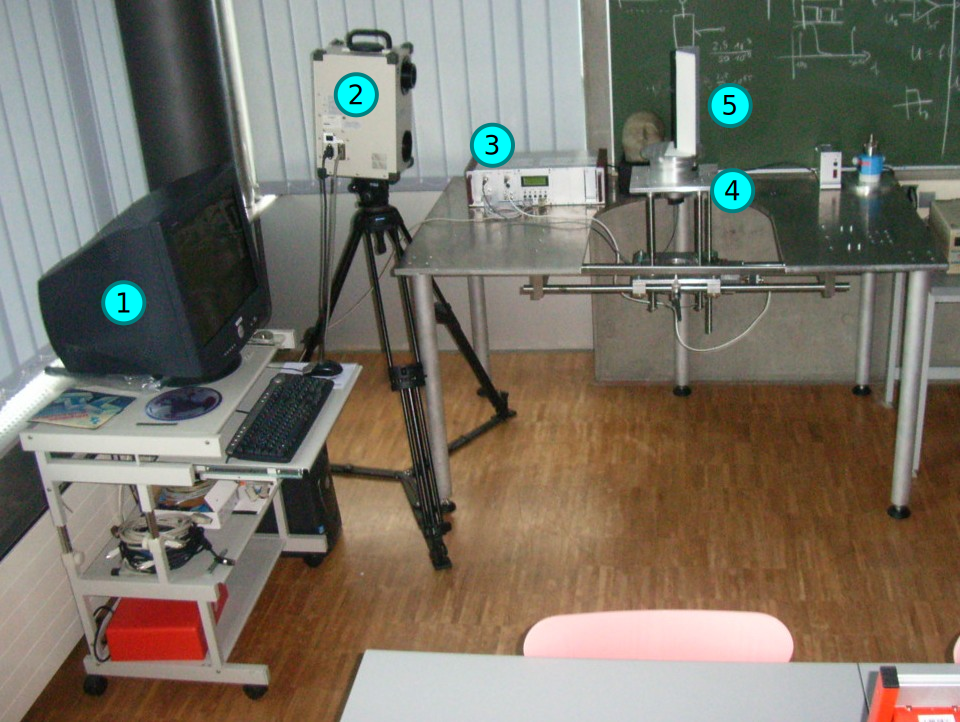
\includegraphics[width=\textwidth]{Uebersicht_2.pdf}
\caption{Blick auf den Arbeitsaufbau}
\label{fig:Übersicht}
\end{figure}
\begin{table}[htb]
\caption{Komponenten im Aufbau}
\begin{tabular}{|c|l|}	\hline 
\rule[-1ex]{0pt}{2.5ex} 1 & 
Computer\\ \hline 
\rule[-1ex]{0pt}{2.5ex} 2 & 
3D-Laserscanner VI-900\\ \hline 
\rule[-1ex]{0pt}{2.5ex} 3 & 
Ansteuerung für den Drehtisch\\ \hline 
\rule[-1ex]{0pt}{2.5ex} 4 & 
Drehtisch\\ \hline 
\rule[-1ex]{0pt}{2.5ex} 5 & 
Zu scannendes Objekt (Kalibrierblech)\\ \hline 
\end{tabular} 
\label{tbl:Aufbau}
\end{table}
\section{Computer}
\label{sec:Computer}
Zur Verfügung steht ein IBM kompatibler x86 Standard PC mit einer \Fachbegriff{SCSI-} und einer \Fachbegriff{RS-232-Schnittstelle}. Auf diesem ist die Erfassungssoftware \emph{RapidForm2004} [\ref{sec:V_Software}] installiert. Die SCSI Schnittstelle wird zur Kommunikation mit dem 3D-Laserscanner und die RS-232-Schnittstelle zur Kommunikation mit einer Schrittmotorsteuerung genutzt.
\section{3D-Laserscanner VI-900}
\label{sec:VI-900}
Der 3D-Laserscanner \emph{VI-900} der Firma \emph{Konica Minolta}[\ref{sec:V_Hardware}] besteht, wie auf Abbildung \ref{fig:VI900} zu sehen, aus einer Kamera und einem \Fachbegriff{Lasertriangulator}. Das System lässt sich über eine SCSI-Schnittstelle ansprechen und konfigurieren. Zur mobilen Nutzung kann das Gerät auch auf der Rückseite bedient werden. Aufgenommene Daten können auf einer \Fachbegriff{CF-Karte} gespeichert werden. Im Projekt wurde jedoch lediglich die direkte Ansteuerung via SCSI genutzt.\\
Der VI-900 digitalisiert Objekte durch ein Laser-Lichtschnittverfahren. Das vom Objekt reflektierte Licht wird von einer CCD-Flächenkamera erfasst, nach Ermittlung der Distanzwerte (Z-Achse) mittels Laser-Triangulation werden die 3D-Daten erstellt. Der Laserstrahl wird mit Hilfe eines hochpräzisen galvanischen Spiegels über das Objekt projiziert, pro Scan werden 640 x 480 Einzelpunkte erfasst.\cite{Minolta:Einleitung}\\
Die Technischen Daten befinden sich im Anhang in Tabelle \ref{tab:TD_VI-910}
\begin{figure}[htb]
\centering
\includegraphics[width=100pt]{vi900-big.jpg}
\caption{VI-900 - Kamera oben, Lasertriangulator unten}
\label{fig:VI900}
\end{figure}
\subsection{Lasertriangulator Prinzip}
\label{sec:LaserTri}
Ein Lasertriangulator besteht, wie in Abbildung \ref{fig:LaserTriangulator} zu sehen, aus einem Laser, einem Linsensystem und im einfachsten Fall, aus einer Pixeldetektorzeile. Der Laser strahlt auf ein Objekt und je nach Entfernung des Objektes wird das Streulicht unter einem anderen Winkel zurückgestrahlt. Das Streulicht wird durch die Linsen auf den Pixeldetektor abgebildet. Über die Position des Laserspots auf dem Pixeldetektor lässt sich auf die Entfernung des Objektes schließen.
\begin{figure}[h]
\centering
\includegraphics[width=100pt]{Laser-Triangulation.png}
\caption{Prinzip: Laser-Triangulation}
\label{fig:LaserTriangulator}
\end{figure}

\section{Drehtisch und Ansteuerung}
\label{sec:AnsteuerungDrehtisch}
\subsection{Drehtisch}
\label{sec:Drehtisch}
Der Tisch in dem der Drehtisch verbaut ist, ist eine Eigenkonstruktion der Werkstatt des RheinAhrCampus Remagen. Er besteht aus einer massiven Edelstahlarbeitsplatte, welche auf 4 Füßen ruht. Aus dieser ist ein Rechteck mit aufgesetztem Halbkreis ausgeschnitten. In diesem Ausschnitt befindet sich der Drehtisch(siehe Abbildung \ref{fig:Drehtisch}). Er ist auf einem Schienensystem gelagert. Mit dem Schienensystem kann der Drehtisch in der Vertikalen positioniert werden. Mit einem Schrittmotor lässt sich der Drehtisch zusätzlich in der Höhe verstellen. Die Höhenverstellung wird mit einem \Fachbegriff{Schneckengetriebe} realisiert. Ein weiterer Schrittmotor ist für die Drehung des Tisches zuständig. Der Tisch ist über ein \Fachbegriff{Harmonic-Drive-Getriebe} mit dem Schrittmotor verbunden. Das Übersetzungsverhältnis des Getriebes beträgt 1:50.  
\begin{figure}[h]
\centering
\includegraphics[width=\textwidth]{Drehtisch}
\caption{Drehtisch}
\label{fig:Drehtisch}
\end{figure}
 
\subsection{Spannungsversorgung}
\label{sec:Spannungsv}
Die Schrittmotorkarten werden von einem PC-Netzteil gespeist. Die \Fachbegriff{Logikbausteine} werden mit 5V gespeist, zusätzlich werden die Schrittmotorkarten mit 12V für die Schrittmotoren gespeist. Die Kabel sind direkt an die Verbindungsleisten gelötet.\\
Dies verhindert das einfache Ausbauen der Spannungsversorgung und die einfache Erweiterung um neue Einschubkarten.
\subsection{Schrittmotoren}
\label{sec:Schrittmotoren}
Für die Rotation kommt der Schrittmotor 440-458 der Firma R+S zum Einsatz. Dieser hat einen Schrittwinkel von 1,8°, eine Haltedrehmoment von 500mNm, wird mit 8-Drahtleitung verschaltet und mit 12V Gleichspannung versorgt. Aus dem Schrittwinkel ergeben sich 200 Schritte pro Umdrehung. Diese werden mit einem \Fachbegriff{Harmonic-Drive-Getriebe}, mit einer Übersetzung von 500:1, auf 100.000 Schritte pro Umdrehung erhöht.\\
Für die Höhenverstellung wird der Schrittmotor 440-420, ebenfalls von der Firma R+S, verwendet. Dieser hat auch einen Schrittwinkel von 1,8°, hat jedoch ein Haltemoment von 70mNm, wird in 6-Drahtleitung verschaltet und mit 5V Gleichspannung gespeist. Dieser ist mit einer Übersetzung von 5:1 und einem Schneckengetriebe mit dem Drehtisch verbunden.

\subsection{Schrittmotorkarten}
\label{sec:Schrittmotorkarten}
Die Ansteuerung für die Schrittmotoren sind als 19''-Einschübe realisiert, siehe Abbildung \ref{fig:19Zoll_Rack} links. Für jeden Schrittmotor wird ein Einschub benötigt.
Die Einschübe sind Produkte der Firma R+S. Mittels \Fachbegriff{RS-232 Schnittstelle} lassen sich die Karten konfigurieren und ansteuern. Die Konfiguration und Ansteuerung erfolgt über einen vorgegeben 
\Fachbegriff{ASCII}\footnote{Der American Standard Code for Information Interchange (ASCII, alternativ US-ASCII, oft [æski] ausgesprochen) ist eine 7-Bit-Zeichenkodierung\cite{wiki:ASCII}}
 Befehlssatz. Der Befehlssatz befindet sich im Kapitel \ref{sec:A_ASCII_Befehle}. Es können zwei oder mehr Karten als 
\Fachbegriff{Daisy-Chain}\footnote{Als Daisy Chain (englisch, wörtlich „Gänseblümchenkette“) bezeichnet man eine Anzahl von Hardware-Komponenten, welche in Serie miteinander verbunden sind (meist in sogenannten Bussystemen in der Automatisierungstechnik).\cite{wiki:Daisy} } in Reihe geschaltet werden.\\
Zu Beginn des Projekts war nur die erste Schrittmotorsteuerung vorbereitet.
\begin{figure}[h]
\centering
\includegraphics[width=\textwidth]{19Zoll_Rack}
\caption{Ansteuerung im 19''-Rack}
\label{fig:19Zoll_Rack}
\end{figure}
\subsection{Motorverkabelung}
\label{sec:Motorverkabelung}
Die Schrittmotoren benötigen ein mindestens 4-adriges Kabel. Das Kabel für den Schrittmotor, der für die Rotation zuständig ist, war bereits gefertigt. Ein Kabel zwischen Schrittmotor und Schrittmotorkarte zur Höhenverstellung und für die Endschalter war nicht vorhanden und wurde im Verlauf des Projekts gefertigt. 

\subsection{Endschalter}
\label{sec:Endschalter}
Die Schrittmotorkarten unterstützen das Abschalten der Motoren wenn ein sogenannter Endschalter ausgelöst wird. Dies sind im allgemeinen mechanische Schalter die ausgelöst werden wenn der Tisch sich dem Ende des Arbeitsbereiches nähert. Dies verhindert eine Beschädigung des Aufbaus.\\
Im Aufbau sind bereits induktive Endschalter der Firma \textit{Pepperl+Fuchs} verbaut. Diese werden durch einen Metallstutzen ausgelöst. Dieser ist jedoch schlecht positioniert oder ungenügend lang. Würde der Drehtisch über seine Grenzen hinaus in der Höhe verstellt werden, würden die Endschalter nicht rechtzeitig ausgelöst werden und der Aufbau würde beschädigt werden.


\section{Mikrocontroller}
\label{sec:Mikrocontroller}
Ein Mikrocontroller besteht, wie in Abbildung \ref{fig:uC_Blockdiagramm} zu sehen, aus CPU, Flash-Speicher, EEPROM, Registern, Ports und mehreren Peripherie-Funktionen wie z.B. Timern, ADC, DAC und seriellen Schnittstellen. Für unterschiedliche Aufgaben können unterschiedliche Mikrocontroller verwendet werden, welche sich in ihrem Funktionsumfang unterscheiden.\\
Besonders Wichtig im Mikrocontroller sind die sogenannten Register. Dieses sind spezielle, meist 8-Bit breite, Abschnitte im Speicher. Sie repräsentieren Werte und Einstellungen im Mikrocontroller. Diese können  beschrieben und ausgelesen oder nur ausgelesen werden. Durch das Auslesen oder Beschreiben der Register kann der Mikrocontroller mit internen und externen Komponenten interagieren. Die Register die zur externen Kommunikation dienen werden als Ports bezeichnet. \\
Es stand ein ATmega8515 \cite{atmel:8515} im DIL-Gehäuse zur Verfügung. Dieser hatte 8 Kbyte Flash, drei externe Interrupts, eine serielle Schnittstelle und konnte mit bis zu 16 MHz betrieben werden. 
Dieser war geeignet um sich mit den speziellen Eigenheiten der Mikrocontroller Programmierung vertraut zu machen.
\begin{figure}[htb]
\centering
\includegraphics[width=\textwidth]{Mikrocontroller_Block}
\caption{Block Diagramm: Mikrocontroller ATmega324A\cite{atmel:ug_324A}}
\label{fig:uC_Blockdiagramm}
\end{figure}

\subsection{Entwicklerboard STK500}
\label{sec:STK500}
Um den Mikrocontroller zu programmieren und die Programmierung zu überprüfen, wird das \Fachbegriff{Entwicklerboard} \emph{STK500}[\ref{sec:V_Hardware}], wie auf Abbildung \ref{fig:STK500} zu sehen, verwendet. Das Board enthält mehrere Mikrocontroller-Steckplätze, 2 serielle Schnittstellen, 8 Taster, 8 LEDs, 2 Erweiterungsports, eine \Fachbegriff{ISP}\footnote{In System Programmer} Programmierschnittstelle und mehrere Jumper zum Konfigurieren des Boards.\\
Von den beiden seriellen Schnittstellen kann die Eine zur Programmierung des Mikrocontrollers verwendet werden. Die Andere kann zur Kommunikation mit dem Mikrocontroller genutzt werden.\\
Auf dem Board stehen fünf 10 polige Stiftleisten 
zur Verfügung. Diese sind direkt mit den Ein- und Ausgabe Pins, den sogenannten \emph{Ports}, des Mikrocontroller verbunden und können über Flachbandkabel mit Hardwarekomponenten wie z.B. Taster, LED, LC-Displays oder seriellen Schnittstellen verbunden werden.
\begin{figure}[htb]
\centering
\includegraphics[width=\textwidth]{STK500_Schema.pdf}
\caption{Schemazeichnung eines STK500\cite{atmel:ug_STK500}}
\label{fig:STK500}
\end{figure}

\subsection{AVRISP mkII}
\label{sec:AVRISP}
Der \emph{AVRISP mkII}[\ref{sec:V_Hardware}] ist ein USB-basierter \Fachbegriff{In-System-Programmer}. Dieser kann anstelle des RS-232 basierten Programmiersystem des STK500 verwendet werden.\\
Die Übertragungsgeschwindigkeit des AVRISP mkII ist wesentlich höher als die der seriellen Schnittstelle. 
%Desweiteren wurde der ATmega324A nicht mehr vom STK500 internen ISP unterstützt.\\
Der AVRISP mkII lässt sich einfach an den Programmierport, eine 6-Polige Stiftleiste, des STK500 anschließen.

\subsection{MAX232}
\label{sec:MAX232}
Um die serielle Schnittstelle am Mikrocontroller nutzen zu können, müssen die Spannungspegel auf die des RS-232 Standards gewandelt werden. Dazu befindet sich auf dem STK500 der \Fachbegriff{Pegelwandler} MAX232. 
Dieser wandelt die Spannungspegel des Mikrocontrollers (typ. 0 V -- 5 V \Fachbegriff{TTL}\footnote{Transistor-Transistor-Logik}) auf die Spannungspegel des RS-232 Standards (typ. -12 V -- +12 V).
	% Hardwareentwicklung
\chapter{Vorstellung der vorhandenen Software}
\label{cha:Software}

\section{RapidForm2004}
\label{sec:RapidForm}
Zur Erfassung von 3D-Modellen am PC steht die Software RapidForm2004 der Firma INUS Technology Inc. zur Verfügung. Diese ist zur Erfassung und Bearbeitung von 3D-Modellen gedacht. Sie bietet umfangreiche Möglichkeiten die aufgenommenen Modelle zu verbessern, zu verändern, zu vermessen und in verschiedene Formate zu exportieren.\\
Die Ansteuerung des VI-900 ist durch ein \Fachbegriff{Add-In} bereits in die Software integriert. Das Add-In kann den VI-900 ansteuern und die aufgenommenen Daten auslesen. Weiterhin kann das Add-In verschiedene Drehtische ansteuern.

\section{Entwicklungsumgebung}
\label{sec:Entwicklungsumgebung}
Die von Atmel bereitgestellte Entwicklungsumgebung besteht aus einem Editor, dem Compiler und einer Programmiersoftware. Der Editor bietet Komfortfunktionen wie \Fachbegriff{Syntaxhighlighting}, Autovervollständigung und Projektmanagement.

\section{Terminalprogramme}
\label{sec:Terminal}
Als Terminalprogramm zur Kommunikation zwischen Datengeräten über die serielle Schnittstelle steht das Programm "Hypterminal" der Firma Microsoft zur Verfügung.


%\section{Weiteres}Pins am Mikrcontroller werden wie folgt angegeben PortX(a:b).Das X steht dabei für den Portbuchstaben von A--D. Die Buchstaben a und b stehen für die Pinnummer.\\PortB(3:6) würde also die Pins 3--6 an PortB beschreiben.	% Softwareentwicklung
\chapter{Fazit und weitere Möglichkeiten}
\label{cha:Fazit}
\section{Fazit}
Das vorgegeben Ziel den Aufbau in Betrieb zu nehmen und mit einem Mikrocontroller so zu erweitern, dass die Erfassungssoftware RapidForm2004 kompatibel mit dem vorhandenen Drehtisch ist, wurde erreicht. Die Software kann vollständig genutzt werden und fast alle Funktionen der Schrittmotorsteuerungen werden unterstützt. Im Anhang \ref{sec:StepbyStep} befindet sich eine Schritt-für-Schritt Anleitung mit der auch Laien das System nutzen können.
\section{Bekannte Probleme}
Bei einem abschließenden Test funktionierte das Anzeigen einer Meldung beim erreichen der Endschalter, auf dem Display nicht. Alle Verbindungen sind vorhanden und die Programmierung des Mikrocontrollers vollständig. Das Problem ist nicht bekannt und das Auffinden würde weitere Zeit in Anspruch nehmen.\\
Das Display zeigt während der Rotation \emph{0} anstatt dem Winkel an, um den rotiert wird. Für die Anzahl der Schritte funktionierte diese Anzeige. Vermutlich liegt hier ein Fehler in der Berechnung des Winkels vor.
\section{Weitere Möglichkeiten}
Eine elegantere Lösung als die Befehle der Befehlssätze in einem Array zu speichern wäre es diese in verketteten Pointer Structs zu speichern. Diese Idee kam leider erst gegen Ende des Projektes und konnte daher aus Zeitmangel nicht mehr umgesetzt werden.\\
Im Menü lassen sich zur Zeit nur voreingestellte Winkel bzw. Schrittzahlen auswählen. Hier könnte noch eine Funktion geschrieben werden die es dem Benutzer erlaubt Winkel frei einzustellen.
				% Fazit und Zukunft

% Literaturverzeichnis -----------------------------------------------------
%	Das Literaturverzeichnis wird aus der Datenbank Bibliographie.bib 
% 	erstellt. Die genaue Verwendung von bibtex wird hier jedoch nicht erklärt.
%	Link: http://de.wikipedia.org/wiki/BibTeX
% --------------------------------------------------------------------------
\bibliography{Bibliographie}		% Aufruf: bibtex FHWTVorlage
\bibliographystyle{natdin}			% DIN-Stil des Literaturverzeichnisses
%\chapter*{Erklärung des Autors}
%\addcontentsline{toc}{chapter}{Erklärung des Autors}
\addchap{Eidesstattliche Erklärung}
Ich versichere hiermit, dass ich meine Diplomarbeit mit dem Thema
\begin{quote}
\textit{\titel} \textit{\untertitel}
\end{quote}
selbständig verfasst und keine anderen als die angegebenen Quellen und Hilfsmittel benutzt habe. Die Arbeit wurde bisher keiner anderen Prüfungsbehörde vorgelegt und auch nicht veröffentlicht.

Die Ergebnisse der Arbeit stehen ausschließlich dem auf dem Deckblatt angeführten Unternehmen zur Verfügung (\textbf{Arbeit mit Sperrvermerk}).

Mir ist bekannt, dass ich meine Diplomarbeit zusammen mit dieser Erklärung fristgemäß nach Vergabe des Themas in dreifacher Ausfertigung und gebunden im Prüfungsamt der FHWT abzugeben oder spätestens mit dem Poststempel des Tages, an dem die Frist abläuft, zu senden habe.\\[6ex]

Vechta, den \today


\rule[-0.2cm]{5cm}{0.5pt}

\textsc{\autor} 
			% Selbständigkeitserklärung 

% Anhang -------------------------------------------------------------------
%		Die Inhalte des Anhangs werden analog zu den Kapiteln inkludiert.
%		Dies geschieht in der Datei Anhang.tex
% --------------------------------------------------------------------------
\begin{appendix}
	\clearpage
	\pagenumbering{roman}
	\chapter{Anhang}
\label{sec:Anhang}

% Rand der Aufzählungen in Tabellen anpassen
\setdefaultleftmargin{1em}{}{}{}{}{}

%\appendixtoc
\section{Schritt für Schritt Anleitung}
\label{sec:StepbyStep}
Eine Schritt für Schritt Anleitung zum vollständigen Scannen und exportieren eines 3D-Objektes.

\begin{longtable}{|>{\RaggedRight}m{5cm}|m{8cm}|} 
\caption{Schritt für Schritt Anleitung} 
\label{tab:StepbyStep}
\\ \hline
\multicolumn{2}{|c|}{\textbf{Schritt für Schritt Anleitung}}
\\ \hline 
\endfirsthead


\multicolumn{2}{|c|}%
{{ Fortsetzung }} 
\\ \hline 
%\multicolumn{1}{|c|}{\textbf{Time (s)}} &
%\multicolumn{1}{c|}{\textbf{Triple chosen}} 
%\\ \hline 
\endhead


\multicolumn{2}{|l|}%
{{\textbf{Schritt 1 - Starten von RapidForm2004}}}
\\ \hline
Auf dem Desktop doppelt auf das RapidForm Icon klicken.
& 
\includegraphics[width=8cm]{Anleitung/1_Desktop}
\\ \hline 
 
\multicolumn{2}{|l|}%
{{\textbf{Schritt 2 - Oberfläche von RapidForm2004}}}
\\ \hline
Die Oberfläche unterteilt sich in Menü, Werkzeugleisten, Projektbaum und ??.
Je nach dem welche Ansicht in ?? gewählt ist, verändern sich auch das Menü und die Werkzeugleisten. 
& 
\includegraphics[width=8cm]{Anleitung/2_RapidForm}
\\ \hline  

\pagebreak 





\multicolumn{2}{|l|}%
{{\textbf{Schritt 3 - Starten des ''ADD-IN''}}}
\\ \hline
In der Menüzeile auf 
\textbf{Macro -> Addins -> Konica Minolta VIVID Direct Control Addin v2.6.11}
klicken.
\todo{Schrittmotor verbinden!}
& 
\includegraphics[width=8cm]{Anleitung/3_ADDIN_Menu}
\\ \hline  

\multicolumn{2}{|l|}%
{{\textbf{Schritt 4 - Kalibrieren vorbereiten}}}
\\ \hline
\begin{TippS}Für ein erfolgreiches Zusammenführen der einzelnen Aufnahmen ist die Kalibrierung unerlässlich!\end{TippS}
Auf dem Add-In Panel, unter dem Vorschau Fenster, auf \textbf{Live-Preview} klicken. \linebreak
Das Kalibrierungsblech auf dem Drehtisch positionieren.  \linebreak
Dabei muss der Noppen an der Unterseite des Kalibrierungsblechs in das mittlere Loch des Drehtisches gesteckt werden. Die abgeklebte Seite muss zum VI-900 zeigen.
& 
%\includegraphics[width=8cm]{Anleitung/3_ADDIN_Menu}
Bild?
\\ \hline  

\pagebreak 


\multicolumn{2}{|l|}%
{{\textbf{Schritt 5 - Kalibrieren}}}
\\ \hline
Den Reiter \textbf{VIVID: 1} auswählen.\linebreak
Bei \textbf{Manual Para.} ein Häkchen setzen.\linebreak
Im Feld \textbf{Laser Power} ''23'' eintragen.\linebreak
Auf \textbf{Scan for Calib} klicken.
& 
\includegraphics[width=8cm]{Anleitung/4_Calibration}
\\ \hline  

\multicolumn{2}{|l|}%
{{\textbf{Schritt 6 - Kalibrierungsergebnis}}}
\\ \hline
Das Ergebnis sollte ähnlich zu dem in der rechten Abbildung sein. \linebreak
Falls das Add-In einen Fehler ausgibt, muss das Kalibrierungsblech eventuell anders positioniert werden, der Wert im Feld \textbf{Laser Power} verändert werden oder der Fokus manuell eingestellt werden.\linebreak
War die Kalibrierung erfolgreich können die \emph{Kalibrationsebenen }im \emph{Projektbaum} ausgeblendet werden.
& 
\includegraphics[width=8cm]{Anleitung/4_Calibration_result}
\\ \hline  

\pagebreak 


\multicolumn{2}{|l|}%
{{\textbf{Schritt 7 - StepScan}}}
\\ \hline
Bei \textbf{Manual Para.} das Häkchen entfernen.\linebreak
Zum Reiter \textbf{Step} wechseln.\linebreak
Bei \textbf{Angle Tag} und \textbf{Rotate Table to next Scan position} Häkchen setzen.\linebreak
Bei \textbf{Init. Align in RF Using Rotary Info.} und \textbf{Auto Accept} die Häkchen entfernen.\linebreak
Bei \textbf{Rotation Step} die gewünschte Drehung in Grad eingeben. \linebreak
''45'', ''60'' und ''90'' sind gute Werte.
& 
\includegraphics[width=8cm]{Anleitung/5_StepScan.jpg}
\\ \hline  

\multicolumn{2}{|l|}%
{{\textbf{Schritt 8 - AutoFocus}}}
\\ \hline
Das \emph{Kalibrationsblech} entfernen und durch das zu scannende Objekt ersetzen.\linebreak
Zum Reiter \textbf{Control} wechseln. \linebreak
Auf \textbf{Autofocus} klicken.\linebreak
& 
\includegraphics[width=8cm]{Anleitung/6_AutoFocus}
\\ \hline  

\pagebreak 


\multicolumn{2}{|l|}%
{{\textbf{Schritt 9 - Scan}}}
\\ \hline
Auf \textbf{Scan} klicken. \linebreak
Das Objekt sollte möglichst schon zu erkennen sein und die Farben sich im Mittleren Bereich bewegen. \linebreak
Ansonsten muss mit den Parametern \textbf{Focus} und \textbf{LaserPower gespielt werden.}
\begin{TippS}Die Position des VI-900 darf nach der Kalibrierung nicht mehr verändert werden!\end{TippS}
& 
\includegraphics[width=8cm]{Anleitung/7_Scan}
\\ \hline  

\multicolumn{2}{|l|}%
{{\textbf{Schritt 10 - Akzeptieren}}}
\\ \hline
Wenn das Objekt gut zu erkennen ist, werden mit \textbf{Accept} die Daten an RapidForm2004 gesendet. Der Drehtisch sollte sich nun automatisch um den eingestellten Winkel drehen. 
\begin{TippS}Bei \textbf{AutoAccept} kann nun ein Häkchen gesetzt werden.\end{TippS}
& 
\includegraphics[width=8cm]{Anleitung/8_Accept}
\\ \hline  

\pagebreak 


\multicolumn{2}{|l|}%
{{\textbf{Schritt 11 - Scannen}}}
\\ \hline
Auf \textbf{Scan} klicken.\linebreak
Diesen Schritt wiederholen bis alle Aufnahmen abgeschlossen sind.\linebreak
& 
\includegraphics[width=8cm]{Anleitung/8_AutoAccept}
\\ \hline  

\multicolumn{2}{|l|}%
{{\textbf{Schritt 12 - Ergebnis der Scans}}}
\\ \hline
Nach Abschluss aller Scans dreht der Tisch sich automatisch in die Ursprungsposition zurück.\linebreak
Im Arbeitsbereich sollten sich nun alle Scans befinden.
& 
\includegraphics[width=8cm]{Anleitung/9_1_Scan_result}
\\ \hline  

\pagebreak 


\multicolumn{2}{|l|}%
{{\textbf{Schritt 13 - Drehen und Zusammenführen der Scans}}}
\\ \hline
In der Menüzeile auf \textbf{Build -> Register -> Rotary Table} klicken.\linebreak
& 
\includegraphics[width=8cm]{Anleitung/10_Rotary_Table}
\\ \hline  

\multicolumn{2}{|l|}%
{{\textbf{Schritt 14 - Registrieren}}}
\\ \hline
Im Dialog auf \textbf{Select Axis} klicken.\linebreak
Im Darstellungsbereich auf die Achse aus dem Kalibrationsscan klicken.
Bei \textbf{Rotation-Angle} den Winkel eines Scans eintragen.\linebreak
Im \emph{Projektbaum} den Entsprechenden Scan auswählen.\linebreak
Die letzten beiden Schritte mit allen Scans wiederholen.\linebreak
Den Dialog mit \textbf{Ok} verlassen.
& 
\includegraphics[width=8cm]{Anleitung/11_Register_Dialog_2}
\\ \hline  

\pagebreak 
 

\multicolumn{2}{|l|}%
{{\textbf{Schritt 15 - Ergebnis}}}
\\ \hline
Als Ergebnis sollte nun ein komplettes 3D-Modell des Objektes herauskommen.
& 
\includegraphics[width=8cm]{Anleitung/11_Register_result}
\\ \hline  




\end{longtable} 


\section{Befehlssatz der vorhandene Schrittmotorkarte}
Tabelle \ref{tbl:ASCII_RS} zeigt den ASCII Befehlssatz der Schrittmotorkarte.
\label{sec:A_ASCII_Befehle}

\begin{table}[htb]
\begin{tabular}{|l|l|}	\hline 
\rule[-1ex]{0pt}{2.5ex} \_A 		& Motorstatus liefern                          \\ \hline 
\rule[-1ex]{0pt}{2.5ex} \_C n		& konstante Geschwindigkeit einstellen         \\ \hline 
\rule[-1ex]{0pt}{2.5ex} \_D n 		& Bezugswert definieren                        \\ \hline 
\rule[-1ex]{0pt}{2.5ex} \_E n		& Motorstrom einstellen                        \\ \hline 
\rule[-1ex]{0pt}{2.5ex} \_F 		& Standardeinstellungen aktivieren             \\ \hline 
\rule[-1ex]{0pt}{2.5ex} \_H 		& Sanfter stop                                 \\ \hline 
\rule[-1ex]{0pt}{2.5ex} \_I 		& 4-Bit-Eingang lesen                          \\ \hline 
\rule[-1ex]{0pt}{2.5ex} \_J jdss 	& Joystickparameter einstellen                 \\ \hline 
\rule[-1ex]{0pt}{2.5ex} \_L n 		& lokalen Modus aktivieren/beenden             \\ \hline 
\rule[-1ex]{0pt}{2.5ex} \_M n 		& n Schritte ausführen                         \\ \hline 
\rule[-1ex]{0pt}{2.5ex} \_MA n 		& zu n bewegen                                 \\ \hline 
\rule[-1ex]{0pt}{2.5ex} \_MC n 		& mit konstanter Geschwindigkeit bewegen       \\ \hline 
\rule[-1ex]{0pt}{2.5ex} \_MCA n 	& MA mit konstanter Geschwindigkeit            \\ \hline 
\rule[-1ex]{0pt}{2.5ex} \_MCL n 	& MC zu Endschalterposition                    \\ \hline 
\rule[-1ex]{0pt}{2.5ex} \_ML n 		& zur Endschalterposition bewegen              \\ \hline 
\rule[-1ex]{0pt}{2.5ex} \_N n 		& Zeilenvorschub (LF, hex. 0A) einfügen/löschen\\ \hline 
\rule[-1ex]{0pt}{2.5ex} \_O n 		& n an 4-Bit-Ausgang senden                    \\ \hline 
\rule[-1ex]{0pt}{2.5ex} \_P nnnn 	& Motorparameter einstellen                    \\ \hline 
\rule[-1ex]{0pt}{2.5ex} \_Q 		& Parameter in EEROM speichern                 \\ \hline 
\rule[-1ex]{0pt}{2.5ex} \_R n 		& Mikroschritteilung einstellen                \\ \hline 
\rule[-1ex]{0pt}{2.5ex} \_RL 		& Endschalterwerte lesen                       \\ \hline 
\rule[-1ex]{0pt}{2.5ex} \_RS  		& verbleibende Schritte lesen                  \\ \hline 
\rule[-1ex]{0pt}{2.5ex} \_S   		& Nothalt                                      \\ \hline 
\rule[-1ex]{0pt}{2.5ex} \_T n 		& Eingang n auslösen                           \\ \hline 
\rule[-1ex]{0pt}{2.5ex} \_W   		& Position anfordern                           \\ \hline 
\end{tabular} 
\caption{ASCII Befehlssatz R+S Schrittmotorsteuerung}\cite{rs:ug_stepper}
Der ''\_''  wird mit der anzusteuernden Kartennummer ersetzt. Dabei wird von 1 aufwärts gezählt. Bei der ersten Karte kann die Nummer weggelassen werden.
\label{tbl:ASCII_RS}
\end{table}



\section{Protokolle aus RapidForm2004}
\lstset{language=Java, basicstyle=\footnotesize, showstringspaces=false, tabsize=8}
\lstinputlisting[label=lst:Protokolle_RF, caption=RapidForm2004 Protokolle Empfang]{Code/Protokolle_RF.txt}

\section{Technische Daten VI-910}
Die Technischen Daten beziehen sich auf den VI-910. Dies ist das Nachfolgemodell. Die meisten Daten sollten jedoch ähnlich sein.
\begin{longtable}{|m{4cm}|m{9cm}|} 
\caption{Technische Daten - VI-910} \\
\hline
\label{tab:TD_VI-910}
Modellbezeichnung & Optischer 3D-Scanner VI-910
 \\ \hline 
Messverfahren & Triangulation durch Lichtschnittverfahren
 \\ \hline 
Autofokus & Autofokus auf Objektoberfläche (Kontrastverfahren);  aktiver AF
 \\ \hline 
Objektive \newline  (wechselbar) & TELE Brennweite f=25mm  \newline 
MITTEL: Brennweite f=14 mm  \newline 
WEIT: Brennweite f=8mm
 \\ \hline 
Messabstand & 0,6 bis 2,5m (2m für WIDE-Objektiv)
 \\ \hline 
Optimaler Messabstand	 & 0,6 bis 1,2m
 \\ \hline 
Laserklasse & Class 2 (IEC60825-1), Class 1 (FDA)
 \\ \hline 
Laser-Scanverfahren	 & Galvanisch-angetriebener Drehspiegel
 \\ \hline 
Messbereich in  \newline X-Richtung (anhängig vom Anstand) & 111 bis 463mm (TELE),  \newline 198 bis 823mm (MITTEL), \newline  359 bis 1.196mm (WEIT)
 \\ \hline 
Messbereich in Y-Richtung (abhängig vom Abstand) & 83 bis 347mm (TELE), \newline  148 bis 618mm (MITTEL),  \newline 269 bis 897mm (WEIT)
 \\ \hline 
Messbereich in Z-Richtung (abhängig vom Abstand) & 40 bis 500mm (TELE), \newline  70 bis 800mm (MITTEL),  \newline 110 bis 750mm (WEIT/Modus FINE)
 \\ \hline 
Genauigkeit	 & X: ±0,22mm, Y: ±0,16mm, Z: ±0,10mm zur Z-Referenzebene (Bedingungen: TELE/Modus FINE , Konica Minolta Standard)
 \\ \hline 
Aufnahmezeit & 0,3s (Modus FAST), 2,5s (Modus FINE), 0,5s (COLOR)
 \\ \hline 
Übertragungszeit zum Host-Computer	 & ca. 1s (Modus FAST) oder 1,5s (Modus FINE)
 \\ \hline 
Scanumgebung, Beleuchtungsbedingungen	 & 500 lx oder geringer
 \\ \hline 
Aufnahmeeinheit & 3D-Daten: 1/3" CCD-Bildsensor (340.000 Pixel) 
Farbdaten: Zusammen mit 3D-Daten (Farbtrennung durch Drehfilter)
 \\ \hline 
Anzahl aufgenommener Punkte	 & 3D-Daten: 307.000 (Modus FINE), 76.800 (Modus FAST) 
Farbdaten: 640 × 480 × 24 Bit Farbtiefe
 \\ \hline 
Ausgabeformat & 3D-Daten: Konica Minolta Format, (STL, DXF, OBJ, ASCII-Punkte, VRML; Konvertierung in 3D-Daten durch Polygon Editing-Software / Standardzubehör)
Farbdaten: RGB 24-Bit Rasterscan-Daten
 \\ \hline 
Speichermedium & Compact Flash Memory Card (128MB)
 \\ \hline 
Dateigrößen & 3D- und Farbdaten (kombiniert): 1,6MB (Modus FAST) pro Datensatz, 3,6MB (Modus FINE) pro Datensatz 
 \\ \hline 
Monitor & 5,7"-LCD (320 × 240 Pixel)
 \\ \hline 
Datenschnittstelle & SCSI II (DMA-Synchronübertragung)
 \\ \hline 
Stromversorgung & Normale Wechselstromversorgung, 100V bis 240 V (50 oder 60 Hz), Nennstrom 0,6 A (bei 100 V) \\ \hline 
Abmessungen (B x H x T)	 & 213 × 413 × 271mm 
 \\ \hline 
Gewicht & ca. 11kg
 \\ \hline 
Zulässige Umgebungsbedingungen (Betrieb) & 10 bis 40°C; relative Luftfeuchtigkeit 65\% oder niedriger (keine Kondensation)
 \\ \hline 
Zulässige Umgebungsbedingungen (Lagerung) & -10 bis 50°C, relative Luftfeuchtigkeit 85\% oder niedriger (bei 35°C, keine Kondensation) 
 \\ \hline 
\end{longtable} 
%\include{Inhalt/uCGrundlagen}
%\include{Inhalt/RS232Grundlagen}
\section{Vom Autor verwendete Software}
\label{sec:Werkzeuge}
Hier ist die verwendete Software aufgelistet. Soweit es möglich war, wurden Open-Source-Programme eingesetzt.
\todo{Überarbeiten!!!}
\begin{itemize}
\item \textbf{RapidForm2004} \\
asdf
\item \textbf{AVRStudio 5} \\
Atmel. \\
Website: \url{http://www.atmel.com/}  
\item \textbf{Eclipse} \\
Eclipse mit CDT und AVRPlugin
\\
Website: \url{http://www.eclipse.org/}  
\item \textbf{AVRDude} \\
Prorammer \\
\todo{Weitere?!}
\end{itemize}

\section{Codelistings}
\subsection{main.c}
\lstset{language=Java, basicstyle=\footnotesize, showstringspaces=false, tabsize=4}
\lstinputlisting[label=lst:main,caption=main.c]{../../main_utf8.c}
\section{Credits}
%Ich möchte mich bei den folgenden Personen recht Herzlich bedanken. Herr Prof. Dr. Carstens-Behrens der mir dieses Projekt anbot und mich während dessen zu meiner vollsten Zufriedenheit betreute. Herr Bildhauer der mir bei Fragen immer freundlich zur Verfügung stand. Herr Steimers der mir bei Problemen immer weiterhelfen konnte und der mir mit seiner hervorragenden Ausstattung weiterhelfen konnte wenn die Werkstatt bereits geschlossen hatte und den Praxisbericht korrekturgelesen hat. 
Den folgenden Personen gebührt mein Dank:
\vspace{2cm}
\newcolumntype{R}[1]{>{\raggedleft\arraybackslash}m{#1}}

\begin{table}[h]
	\begin{tabular}[t]{rl}
		\begin{tabular}[t]{r}
			\textbf{Betreuer} 
		\end{tabular} &
		\begin{tabular}[t]{l}
			Prof. Dr. Carstens-Behrens
		\end{tabular}\\
		
		\begin{tabular}[t]{r}
			\textbf{Hilfestellung bei Problemen aller Art} 
		\end{tabular} &
		\begin{tabular}[t]{l}
				Prof. Dr. Carstens-Behrens\\
				Herr Bildhauer \\
				André Steimers \\
				sowie allen weiteren Personen \\
				aus dem Labor bei Herrn Steimers 
		\end{tabular}\\
		
		\begin{tabular}[t]{r}
			\textbf{Lektoren}
		\end{tabular} &
		\begin{tabular}[t]{l}
			André Steimers \\
			Daniel Frank \\
			Sarina Steinke
		\end{tabular} \\
		\begin{tabular}[t]{r}
			\textbf{3D Grafiken}
		\end{tabular} &
		\begin{tabular}[t]{l}
			Benjamin Dielmann
		\end{tabular}
	\end{tabular}
\end{table}

\vspace{12cm}
\begin{center}
\begin{tiny}
Congratulations! You've reached the end.
\end{tiny}
\end{center} %Vorlage, C-B, Bildh, Werkstatt, Steimers und Co.
\end{appendix}


% Index --------------------------------------------------------------------
%	Zum Erstellen eines Index, die folgende Zeile auskommentieren.
% --------------------------------------------------------------------------
\printindex		% Index hier einfügen

\end{document}
